\documentclass{TIJMUjiaoanSY}
\pagestyle{empty}

\begin{document}

\kecheng{分子生物计算}
\shiyan{实验1 \ Markdown标记语言}
\jiaoshi{伊现富}
\zhicheng{讲师}
\riqi{2016年11月10日10:00-12:00}
\duixiang{生物医学工程与技术学院2013级生信班(本)}
\renshu{30}
\leixing{验证型}
\fenzu{一人一机}
\xueshi{2}
\jiaocai{Perl语言在生物信息学中的应用——基础篇}

\firstHeader
\maketitle
\thispagestyle{empty}

\mudi{
\begin{itemize}
  \item 了解常用的Markdown编辑器。
  \item 熟悉Markdown的扩展语法。
  \item 掌握Markdown的基本语法。
\end{itemize}
}

\fenpei{
\begin{itemize}
  \item (10')Markdown简介:介绍Markdown的基本知识和主要用户。
  \item (10')Markdown编辑器:列举常用的Markdown编辑器。
  \item (80')实验操作:使用Markdown撰写Markdown的语法总结。
\end{itemize}
}

\cailiao{
\begin{itemize}
  \item 主要仪器:一台安装有Markdown编辑器(或联网)的计算机。
\end{itemize}
}
\zhongdian{
\begin{itemize}
  \item 重点难点:Markdown的基本语法。
  \item 解决策略:通过演示进行学习,通过练习熟练掌握。
\end{itemize}
}

\sikao{
\begin{itemize}
  \item 列举常见的Markdown用户。
  \item 列举常见的Markdown编辑器。
  \item 总结Markdown的基本语法。
\end{itemize}
}

\cankao{
\begin{itemize}
  \item Beginning Perl for Bioinformatics, James Tisdall, O'Reilly Media, 2001.
  \item Perl语言入门(第六版),Randal L. Schwartz, brian d foy \& Tom Phoenix著,盛春\ 译,东南大学出版社,2012。
  \item Mastering Perl for Bioinformatics, James Tisdall, O'Reilly Media, 2003.
  \item 维基百科等网络资源。
\end{itemize}
}

\firstTail

\newpage
\otherHeader

\begin{enumerate}
  \item Markdown简介(10分钟)
    \begin{enumerate}
      \item Markdown简介:轻量标记语言,John Gruber,易读易写,书写语言
      \item Markdown用户:Bitbucket,GitHub,Stack Overflow,图灵社区,简书写作网站,为知笔记,……
    \end{enumerate}
  \item Markdown编辑器(10分钟)
    \begin{enumerate}
      \item 本地编辑器:MarkdownPad(Windows),ReText(Linux),Mou(Mac)
      \item 在线编辑器:Cmd Markdown,Markable.in,Dillinger.io
      \item Vim插件:vim-markdown,vim-instant-markdown
    \end{enumerate}
  \item 实验操作(80分钟)
    \begin{enumerate}
      \item 复习Markdown的基本语法
    \begin{figure}[h]
      \centering
      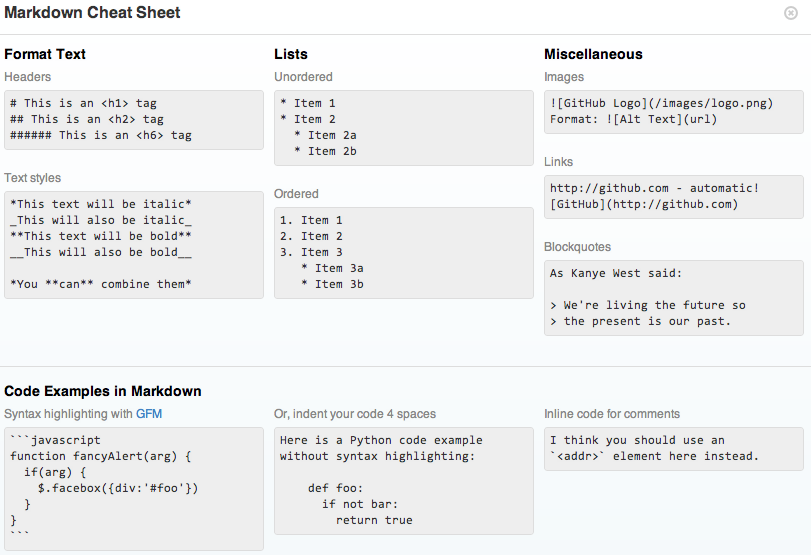
\includegraphics[width=0.9\textwidth]{c1.markdown.cheatsheet.02.png}
    \end{figure}
  \item
    使用Markdown语法撰写Markdown语法的总结报告\textcolor{red}{(尝试在日常生活中使用Markdown,比如:记日记、写作文、整理知识点、做总结报告、……)}
    \end{enumerate}
\end{enumerate}

\otherTail


\end{document}
